\documentclass{article}
\usepackage{tikzpeople}
\usepackage{tikz}
\usetikzlibrary{shapes, shapes.misc}
\usetikzlibrary{arrows, arrows.meta, decorations.markings}
\usetikzlibrary{patterns}

\begin{document}
\begin{center}
\resizebox{\columnwidth}{!}{%
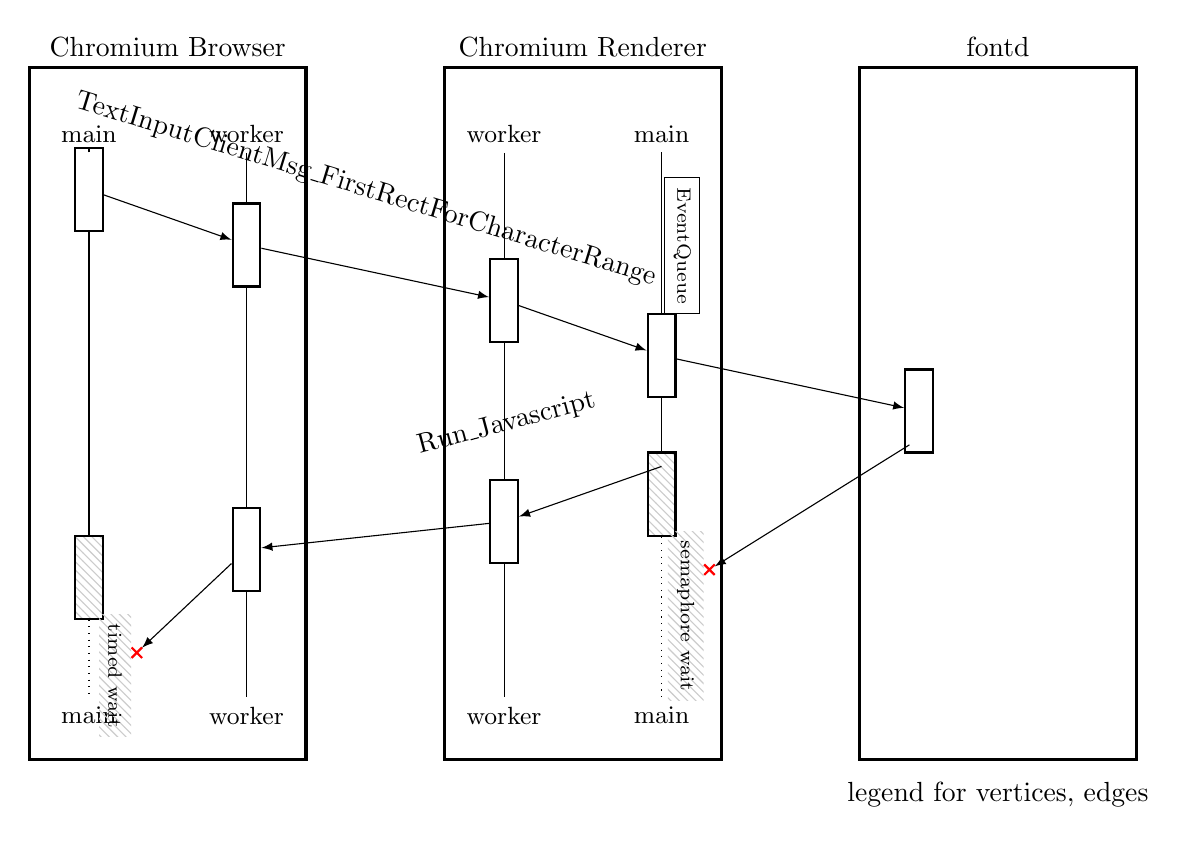
\begin{tikzpicture}[>=latex]
%\tikzstyle{every node}=[font=\Large]
\tikzstyle{app} = [draw, very thick, minimum height=250pt, minimum width=100pt, fill=white, rectangle, font={\sffamily\bfseries}]
\tikzstyle{appbegin} = [minimum width = 20pt, below = -230pt of #1]
\tikzstyle{append} =[minimum width = 20pt, below = -20pt of #1]
\tikzstyle{thread} = [minimum width = 8pt, font=\small]

\tikzstyle{actionpoint} = [draw, thick, minimum width = 10pt, minimum height = 30pt, fill = white]
\tikzstyle{blocked} = [minimum height = 10pt, pattern=north west lines, pattern color = black!20!, font=\scriptsize, rotate=270] 
\tikzstyle{blockedactionpoint} = [draw, thick, minimum width = 10pt, minimum height = 30pt, pattern=north west lines, pattern color = black!20!] 

\tikzstyle{point} = [thick, draw=red, cross out, inner sep = 0pt, minimum width = 3pt, minimum height =3pt]
%\tikzset{
%%ext/.pic={
%%\path [fill=white] (-0.2,0)to[bend left](0,0.1)to[bend right](0.2,0.2)to(0.2,0)to[bend left](0,-0.1)to[bend right](-0.2,-0.2)--cycle;
%%\draw (-0.2,0)to[bend left](0,0.1)to[bend right](0.2,0.2) (0.2,0)to[bend left](0,-0.1)to[bend right](-0.2,-0.2);
%%},
%point/.style={
%    thick,
%    draw=red,
%    cross out,
%    inner sep=0pt,
%    minimum width=4pt,
%    minimum height=4pt,
%}}

%draw applications
%%browser
\node [app, name = browser, label=above:Chromium Browser]{};
\node(browserbegin) [appbegin=browser]{};
\node(browserend) [append=browser]{};
\node (bt1begin)[thread, left of = browserbegin]{main};
\node (bt1end)[thread, left of = browserend]{main}; 
\node (bt2begin)[thread, right of = browserbegin]{worker};
\node (bt2end)[thread,  right of = browserend]{worker};

\node (1)[actionpoint, below of = bt1begin, node distance = 20pt]{};
\node (2)[actionpoint, below of = bt2begin, node distance = 40pt]{};
\node (9)[actionpoint, below of = 2, node distance = 110pt] {};
\node (10)[blockedactionpoint, below of = 1, node distance = 140pt]{};
\node (11)[blocked, below right = -2pt and 10pt of 10]{timed wait};

\draw [solid] (bt1begin) -- (1.north);
\draw [solid] (1.south) -- (10.north);
\draw [dotted] (10.south) -- (bt1end);
\draw [solid] (bt2begin) -- (2.north);
\draw [solid] (2.south) -- (9.north);
\draw [solid] (9.south) -- (bt2end);

%%renderer
\node [app, name = renderer, right of = browser, node distance = 150pt, label=above:Chromium Renderer]{};

\node (rderbegin)[appbegin = renderer]{};
\node (rderend)[append = renderer]{};

\node (rt3begin)[thread, left of = rderbegin]{worker};
\node (rt3end)[thread, left of = rderend]{worker};
\node (rt4begin)[thread, right of = rderbegin]{main};
\node [draw, below right = 9pt and 0.5pt of rt4begin, font=\scriptsize, rotate=270] {EventQueue};
\node (rt4end)[thread, right of = rderend]{main};
%\draw [solid] (bt3begin) -- (bt3end);
%\draw [solid] (bt4begin) -- (bt4end);
\node (3)[actionpoint, below of = rt3begin, node distance = 60pt]{};
\node (4)[actionpoint, below of = rt4begin, node distance = 80pt]{};
\node (7)[blockedactionpoint, below of = 4, node distance = 50pt]{};
\node (12)[blocked, below right = -2pt and 10pt of 7]{semaphore wait};
\node (8)[actionpoint, below of = 3, node distance = 80pt]{};
\draw[solid] (rt3begin) -- (3.north);
\draw[solid] (3.south) -- (8.north);
\draw[solid] (8.south) -- (rt3end);
\draw[solid] (rt4begin) -- (4.north);
\draw[solid] (4.south) -- (7.north);
\draw[dotted] (7.south) -- (rt4end);
%
\node [app, name = fontd, right of = renderer, node distance = 150pt, label=above:fontd]{};
\node (fontdbegin)[appbegin =fontd] {};
\node (fontdend)[append = fontd]{};
\node (ft5begin)[thread, left of = fontdbegin]{};
\node (ft5end)[thread, left of = fontdend]{};
\node (5)[actionpoint, below of = ft5begin, node distance = 100pt] {};
\node (6)[below of = 5, node distance = 10pt] {};
%\draw [solid] (bt5begin) -- (bt5end);
%
\draw [->] (1) -- (2);
\draw [->] (2) -- (3);
\draw [->] (3) -- (4);
\draw [->] (4) -- (5);
\coordinate[name = notarrive7, point, below right = 10pt and 10pt of 7]{};
\draw [->] (6) -- (notarrive7);
\coordinate[name = before7, above of = 7, node distance = 10pt]{};
\draw [->] (before7) -- (8);
\draw [->] (8) -- (9);
\coordinate[name = notarrive10, point, below right = 10pt and 10pt of 10]{};
\draw [->] (9) -- (notarrive10);
%
\node (findfirstrect)[minimum width = 40pt, minimum height = 40pt, right of = 1, node distance = 100pt, rotate= 343] {TextInputClientMsg\_FirstRectForCharacterRange};
\node (javascript)[minimum width = 40pt, minimum height = 40pt, above left = 0pt and 10pt of 7, rotate = 15] {Run\_Javascript};

\node(legend)[ below of = fontdend]{legend for vertices, edges};

\end{tikzpicture}
}
\end{center}
\end{document}
